\section{Evaluation}
We now evaluate the performance of Genesis along various dimensions:
 (1) What is the performance of Genesis in synthesizing simple reachability and waypoint policies
  with increasing number of policies and greater sizes of topologies and benchmarking the constraints used by the synthesis algorithm? 
  (2) How quickly can Genesis synthesize isolation policies in datacenter topologies for varying number of policies and percentage of
   datacenter utilization? 
   (3) What is the performance of Genesis for solving link-capacity policies in internet topologies? 
   (4) Identifying the benefits of tactics in terms of reduction of terms in the synthesis algorithm and actual benefits 
   with respect to synthesis without tactics for different isolation workloads in datacenter topologies? 
   (5) What are the potential speedups of using optimistic synthesis in Genesis for varying workloads? 

\subsection{Reachability and Waypoint Policies}
\begin{figure*}
	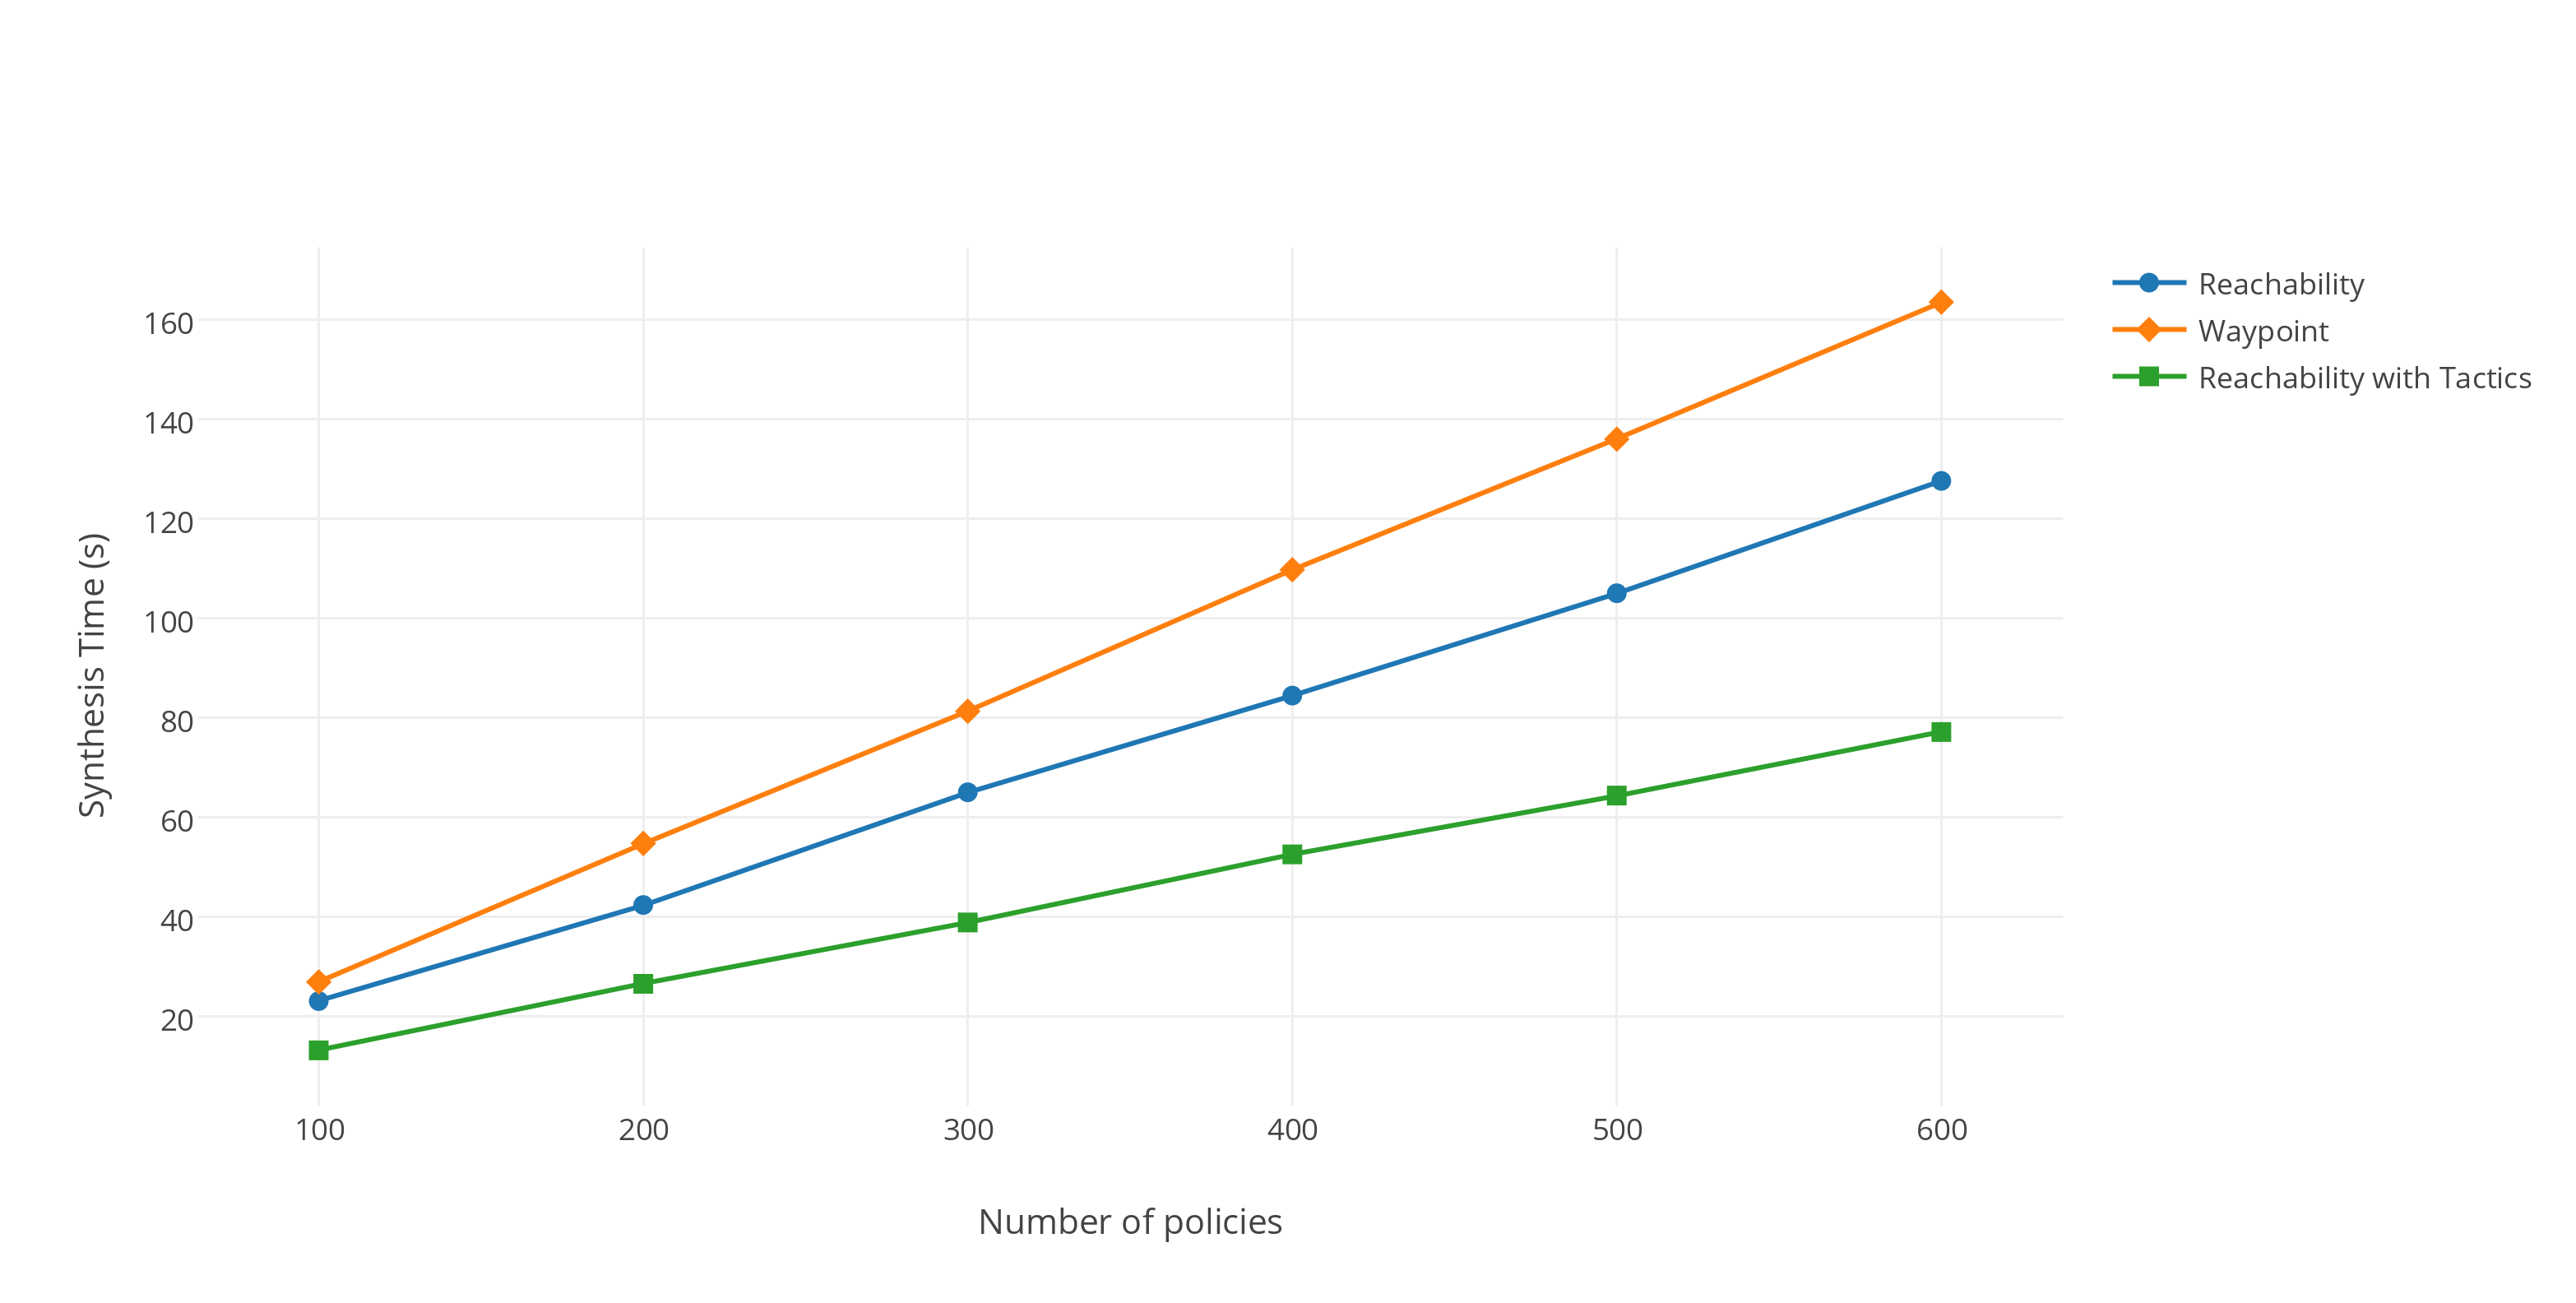
\includegraphics[height=7.5cm]{figures/reach-way-tactic.png}
	\caption{Graph used to compare time taken for reach v/s waypoint policies in a 45-node fat-tree topology and emphasise due to the generality of the approach we cannot solve reachability using classic algorithms. We therefore need a more heavyweight approach that is slowish. The tactic plot is to show improvements of solving reach using a tactic}
	\label{fig:reach-way-tactic}
\end{figure*}
\begin{figure*}
	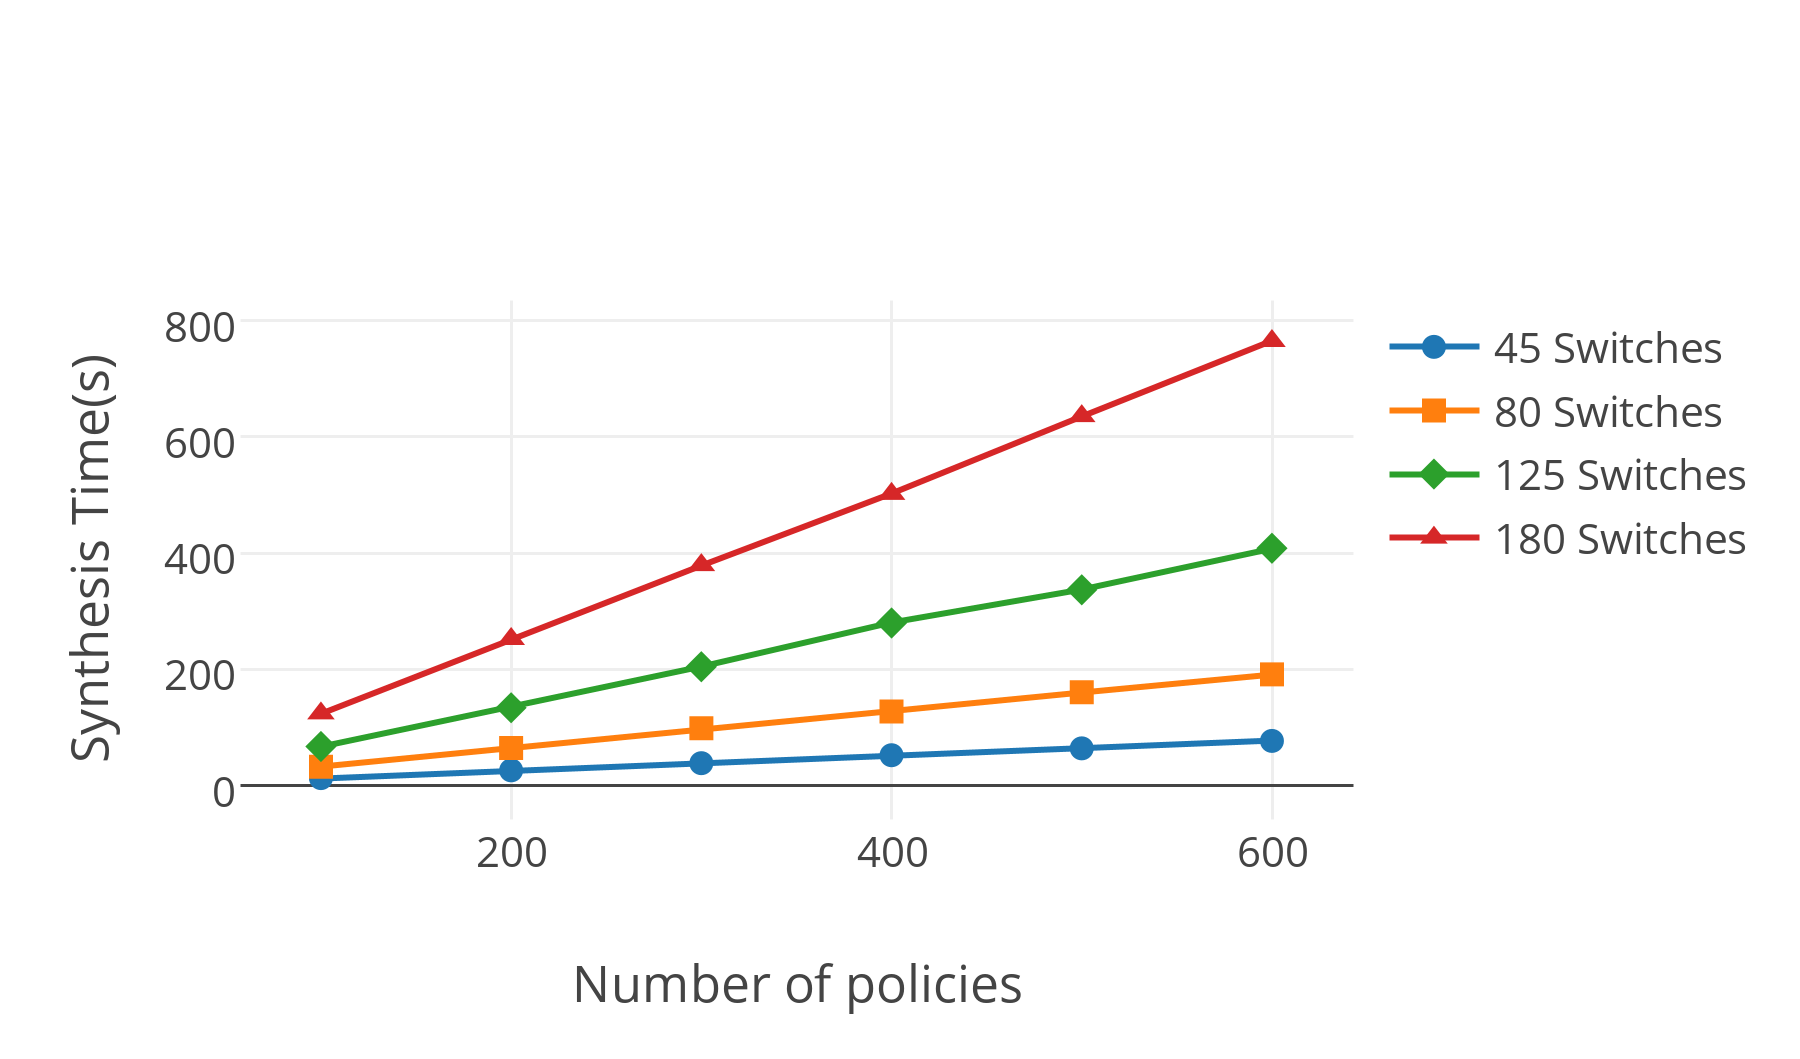
\includegraphics[height=7.5cm]{figures/reach-topo.png}
	\caption{Graph used to compare time taken for reachability policies for varying topology sizes}
	\label{fig:reach-topo}
\end{figure*}

\subsection{Isolation-Policies}
\begin{figure*}
	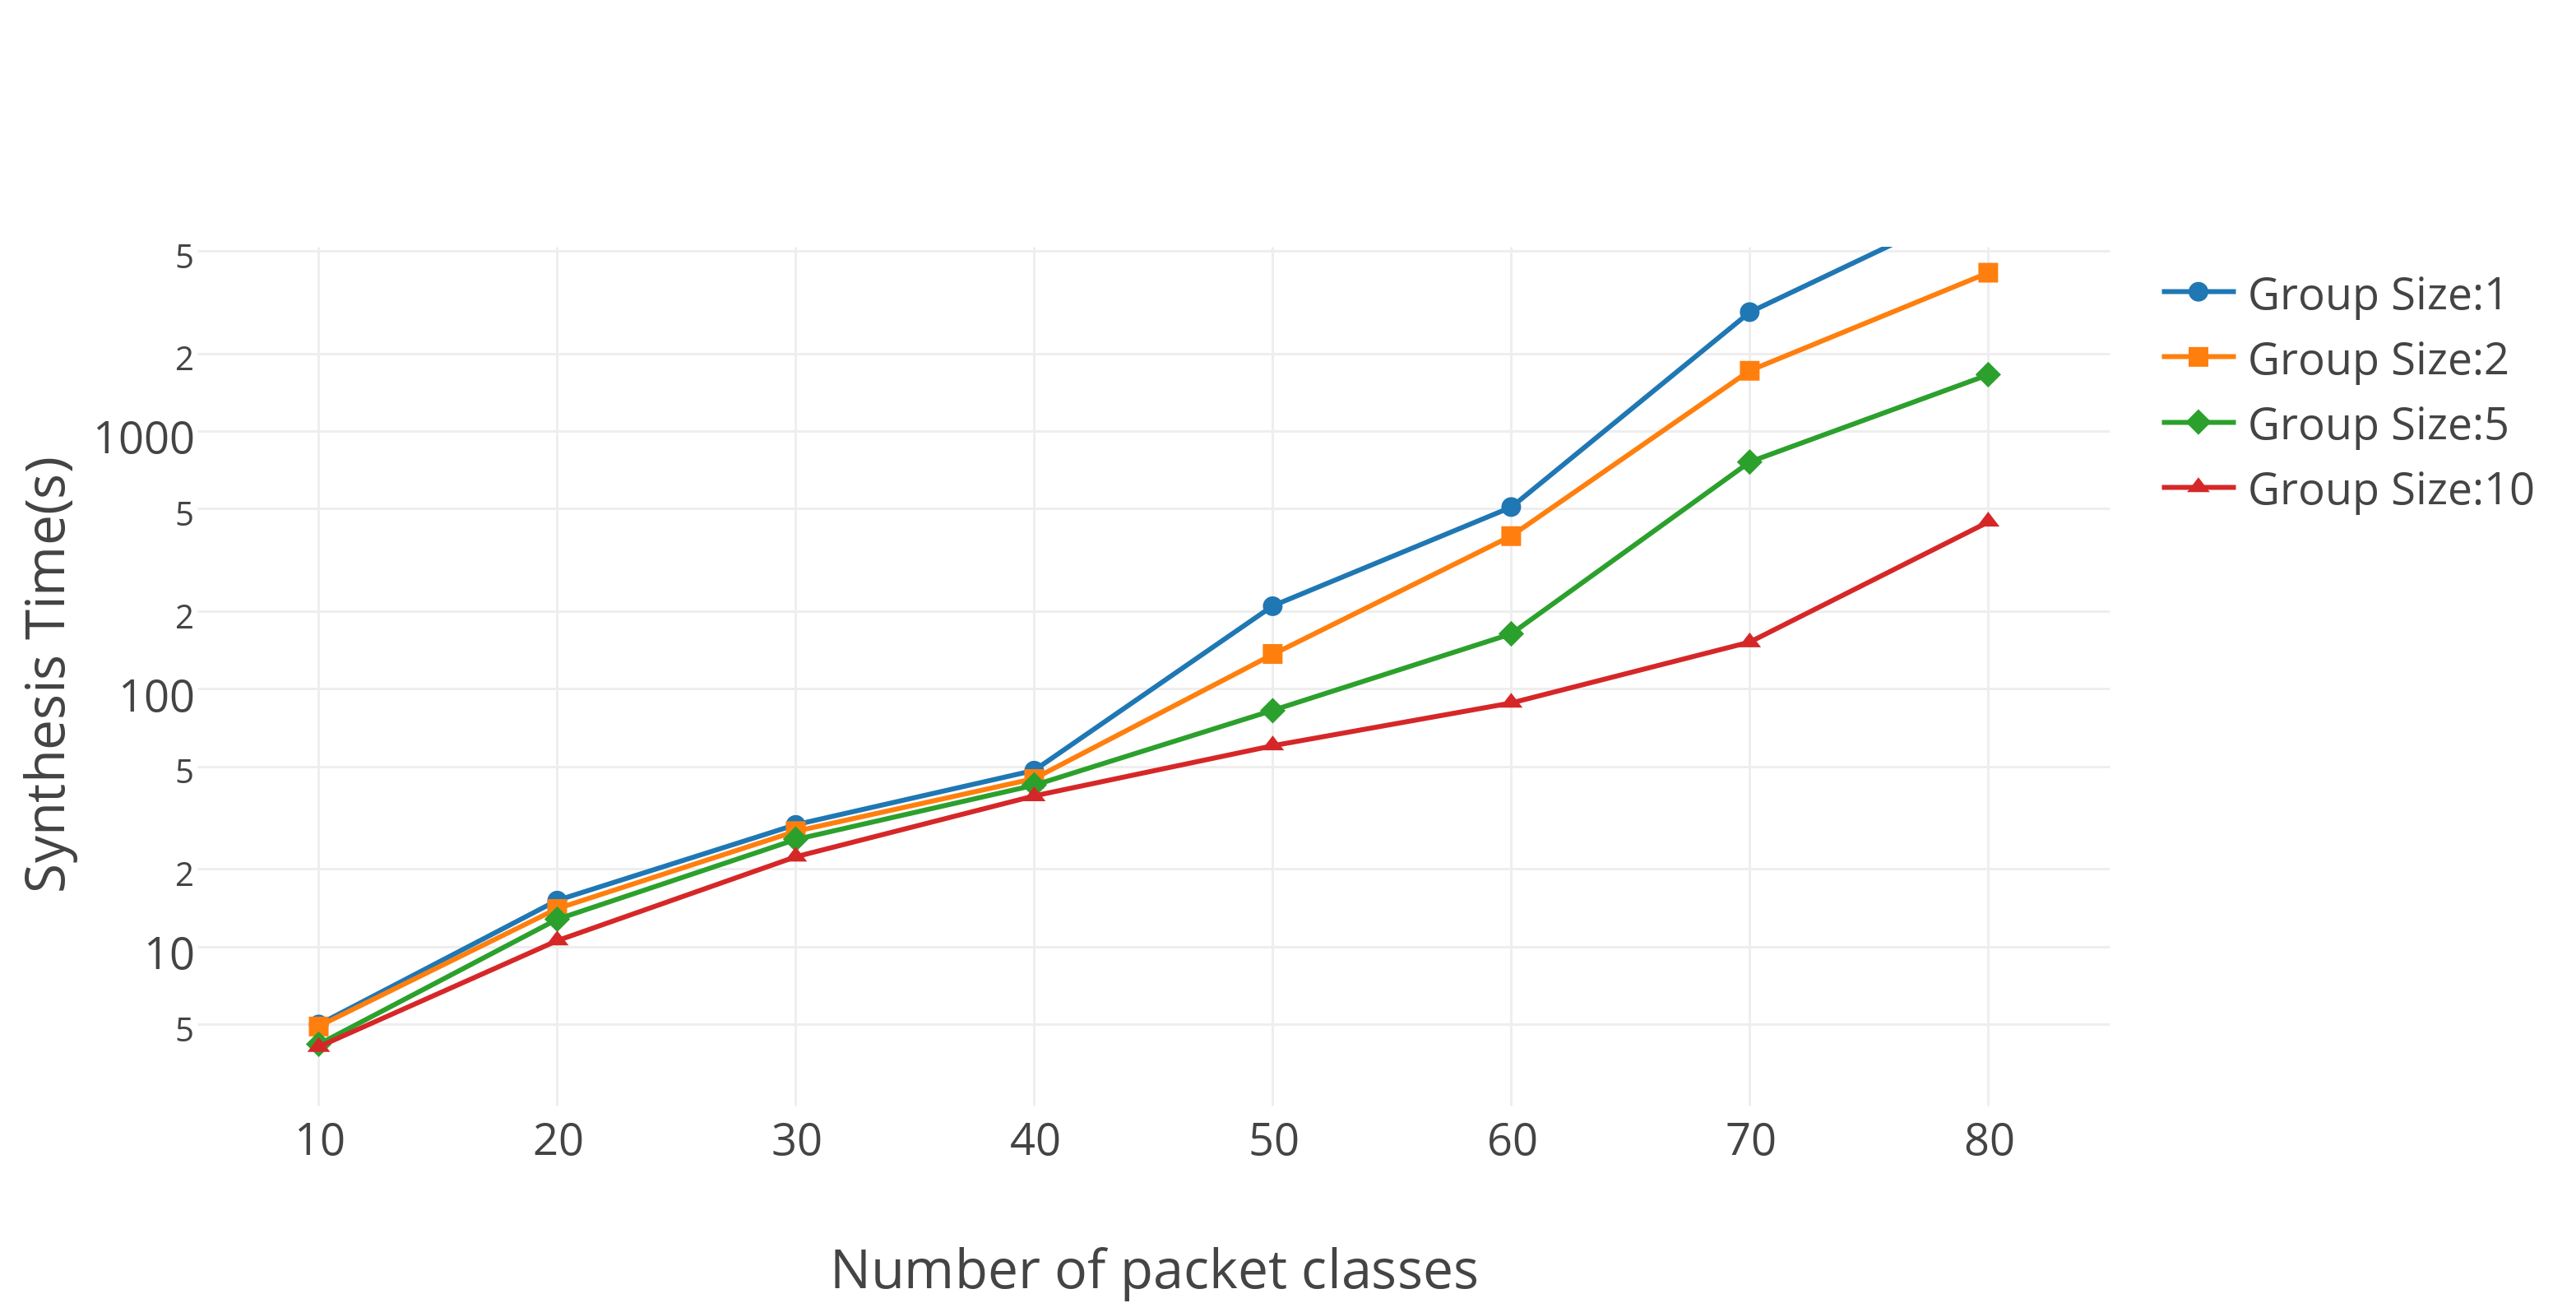
\includegraphics[height=7.5cm]{figures/performance-isolation-groups-log-scale.png}
	\caption{Graph used to compare time taken for solving isolation policies for varying workloads in a 80 node fat-tree topology}
	\label{fig:isolation}
\end{figure*}

\subsection{Link Capacity Policies}


\subsection{Tactic Reductions}
\begin{figure*}
	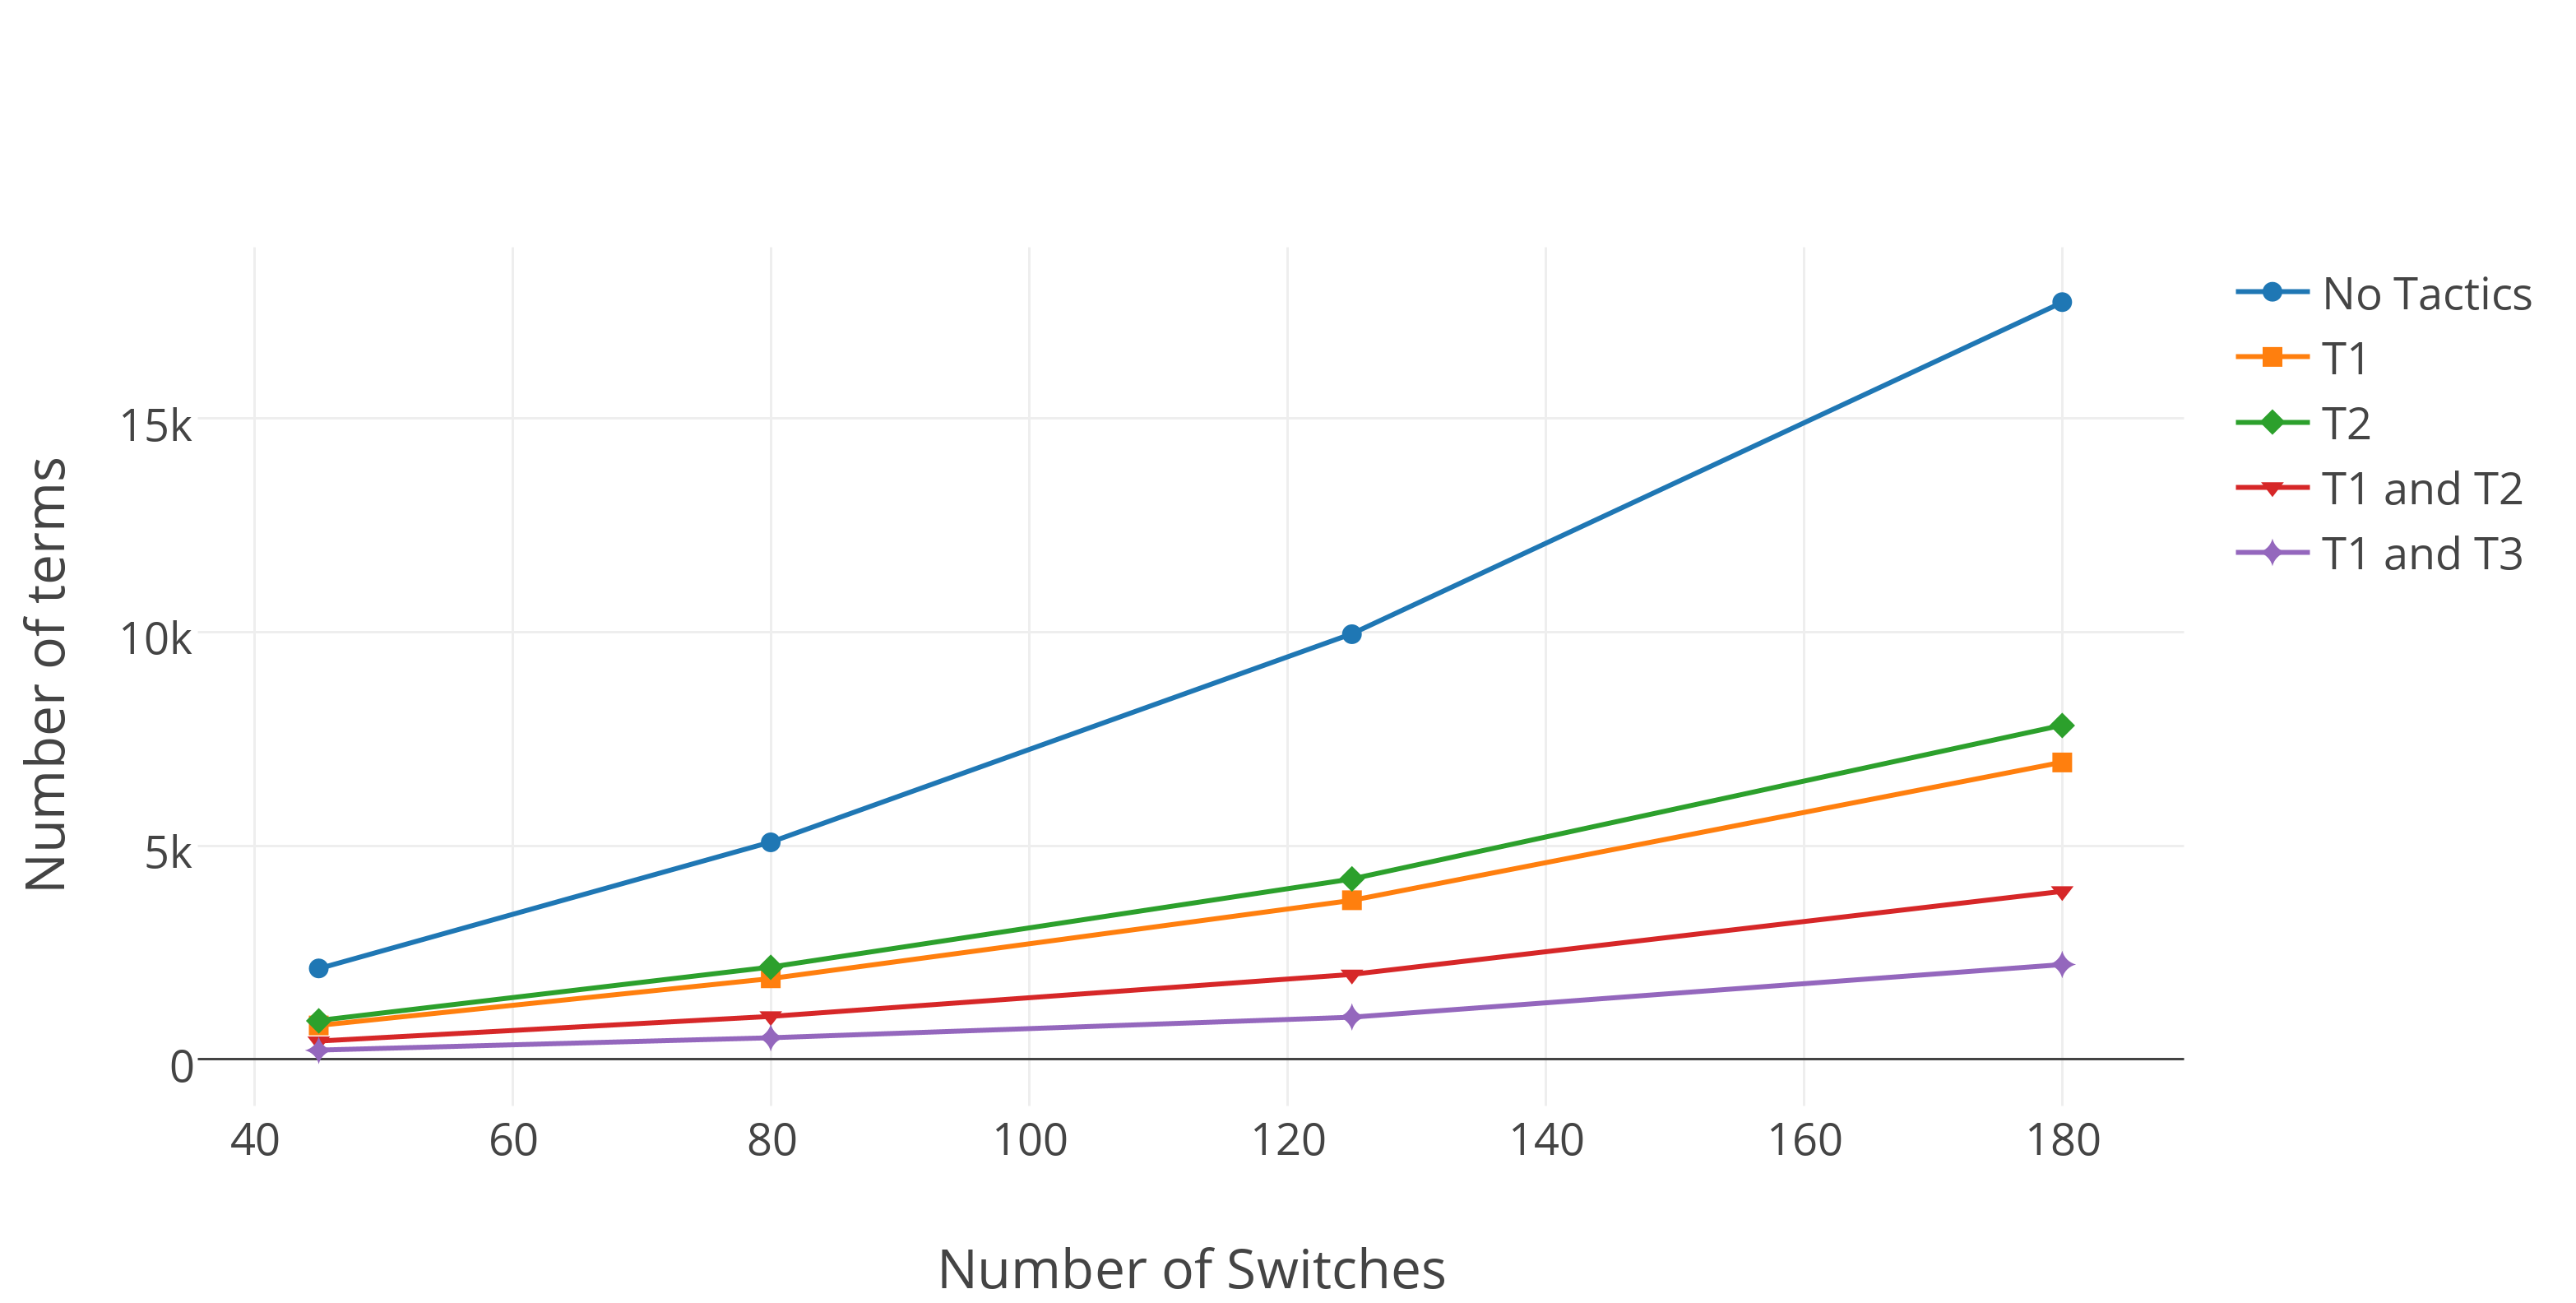
\includegraphics[height=7.5cm]{figures/tactic-reduction.png}
	\caption{Graph used to show the reduction of terms using different tactics w.r.t the total number of terms}
	\label{fig:tactic-reduction}
\end{figure*}

\begin{figure*}
	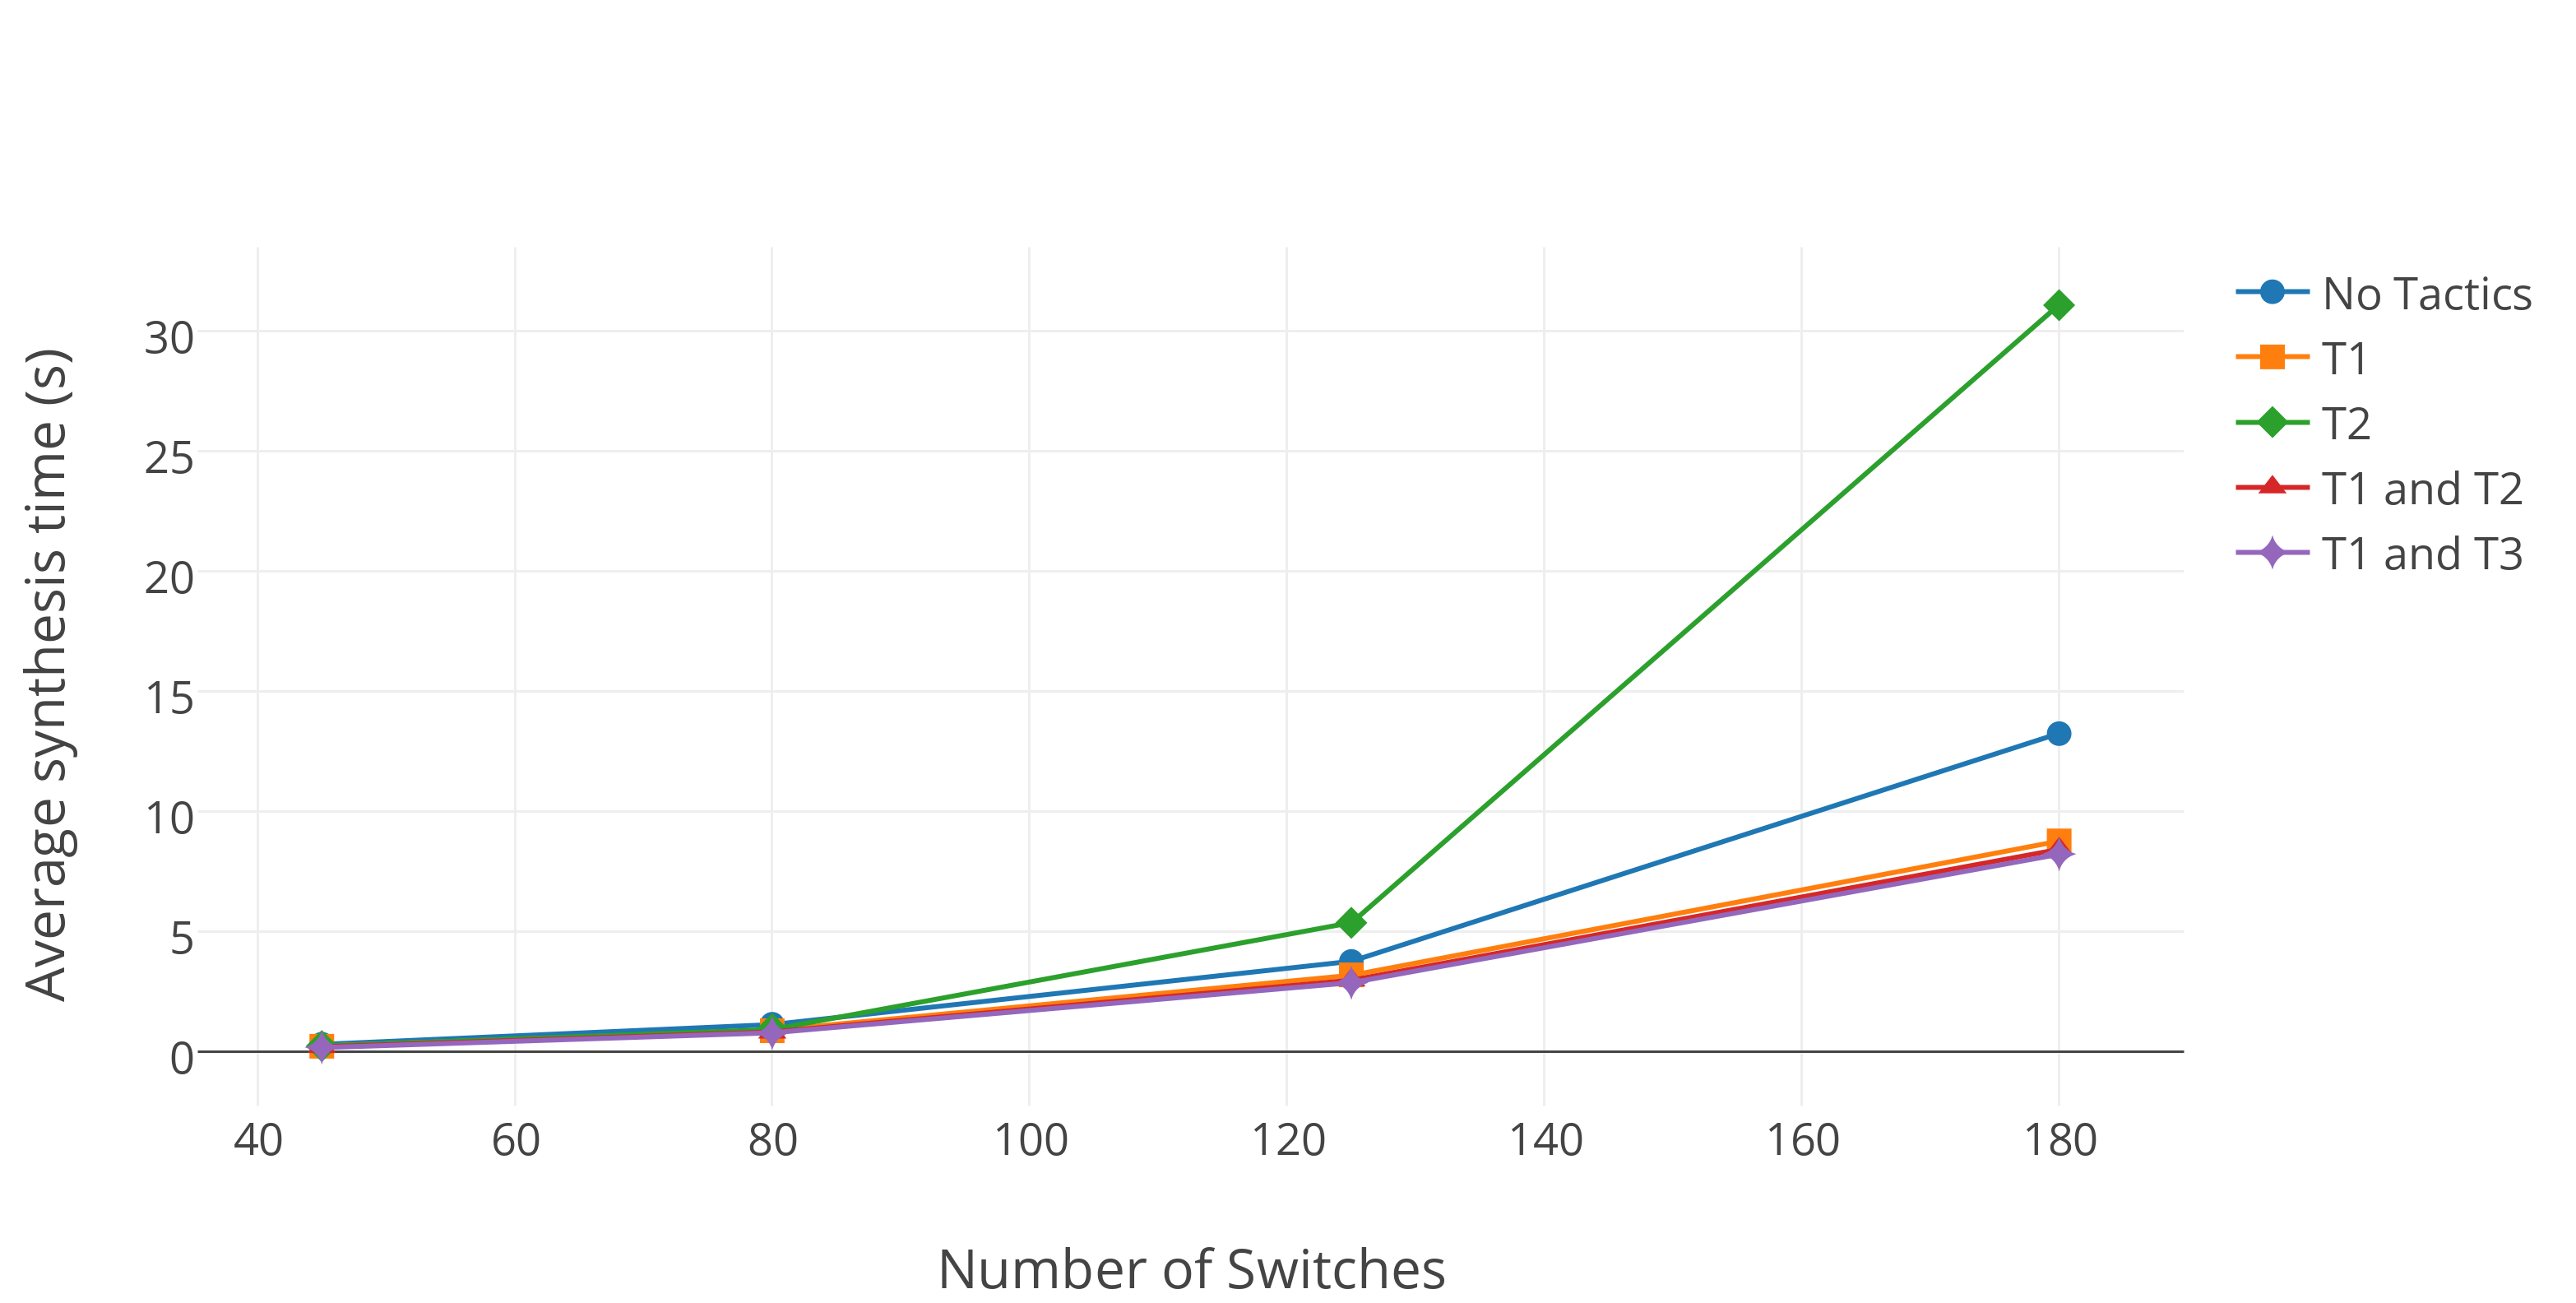
\includegraphics[height=7.5cm]{figures/isolation-tactics.png}
	\caption{Graph used to application of tactics for a isolation workload (percentage isolation w.r.t topology 25\%) and different topology sizes. An interesting observation in the graph is that tactics need not always help in reduction of constraints (One of the tactics, not  a very natural one) leads to more time to synthesis without tactics.}
	\label{fig:isolation-tactics}
\end{figure*}

\subsection{Optimistic Synthesis}
\begin{figure*}
	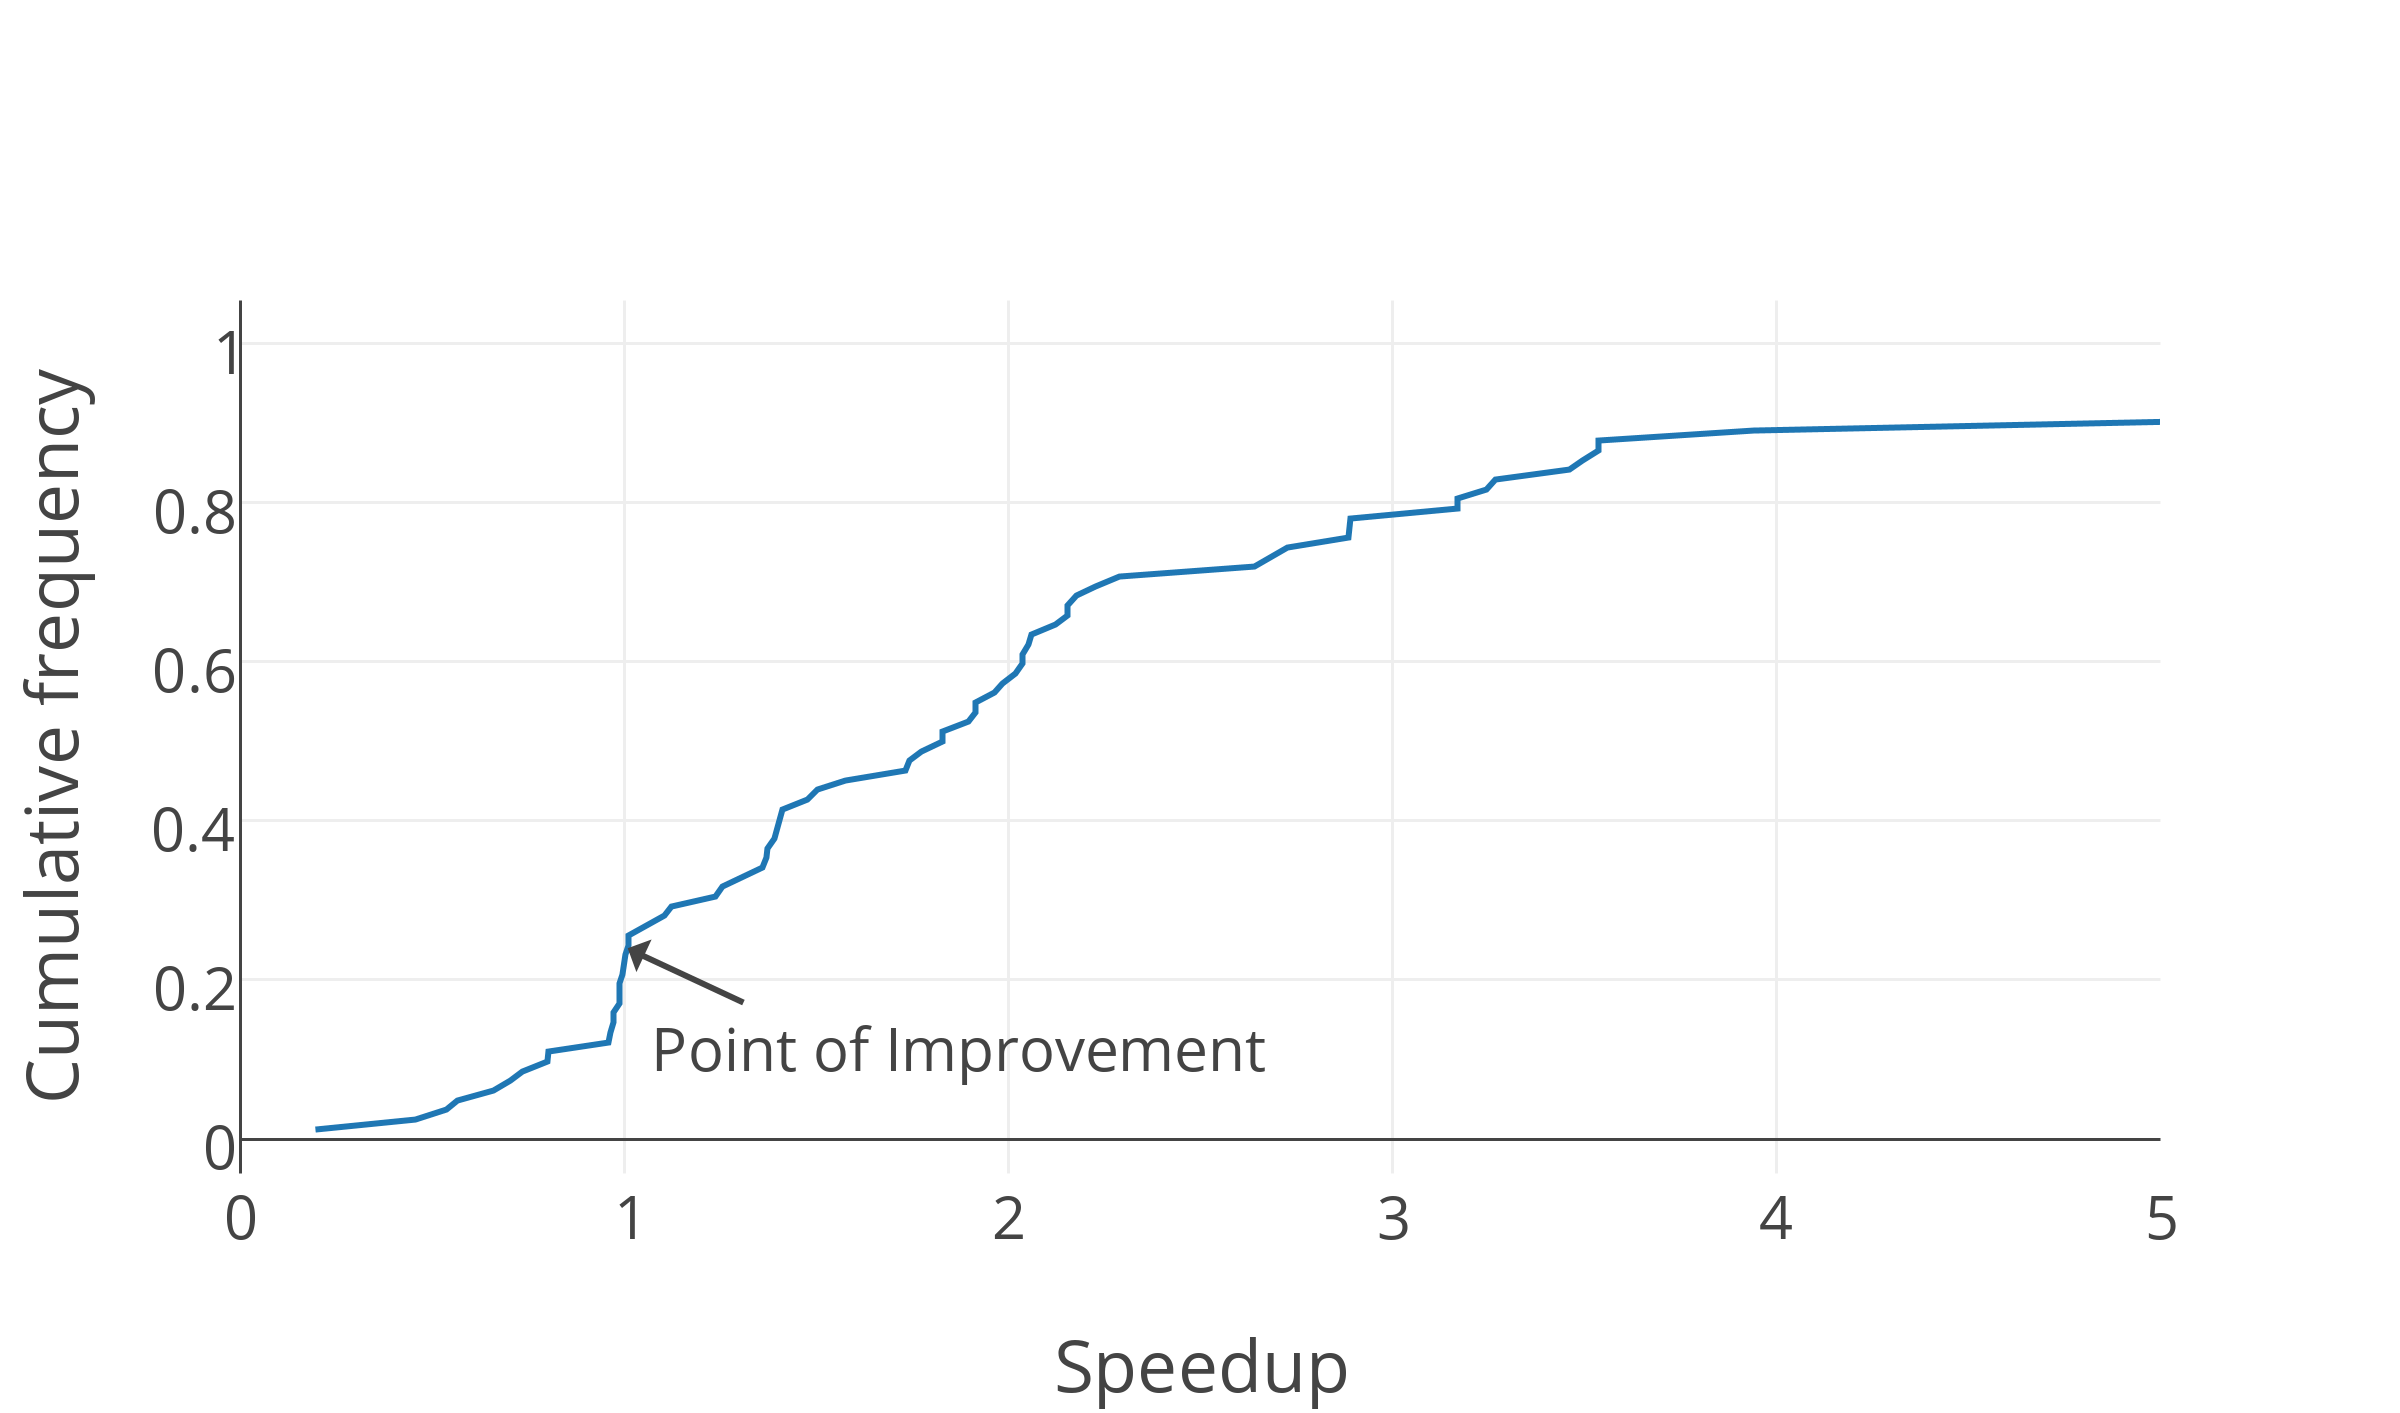
\includegraphics[height=7.5cm]{figures/opt-cdf.png}
	\caption{Graph used to plot the cummulative frequency for speedup achieved by optimistic synthesis (Speedup = optimistic/normal)}
	\label{fig:opt-cdf}
\end{figure*}

\subsection{Incremental Synthesis}
\begin{figure*}
	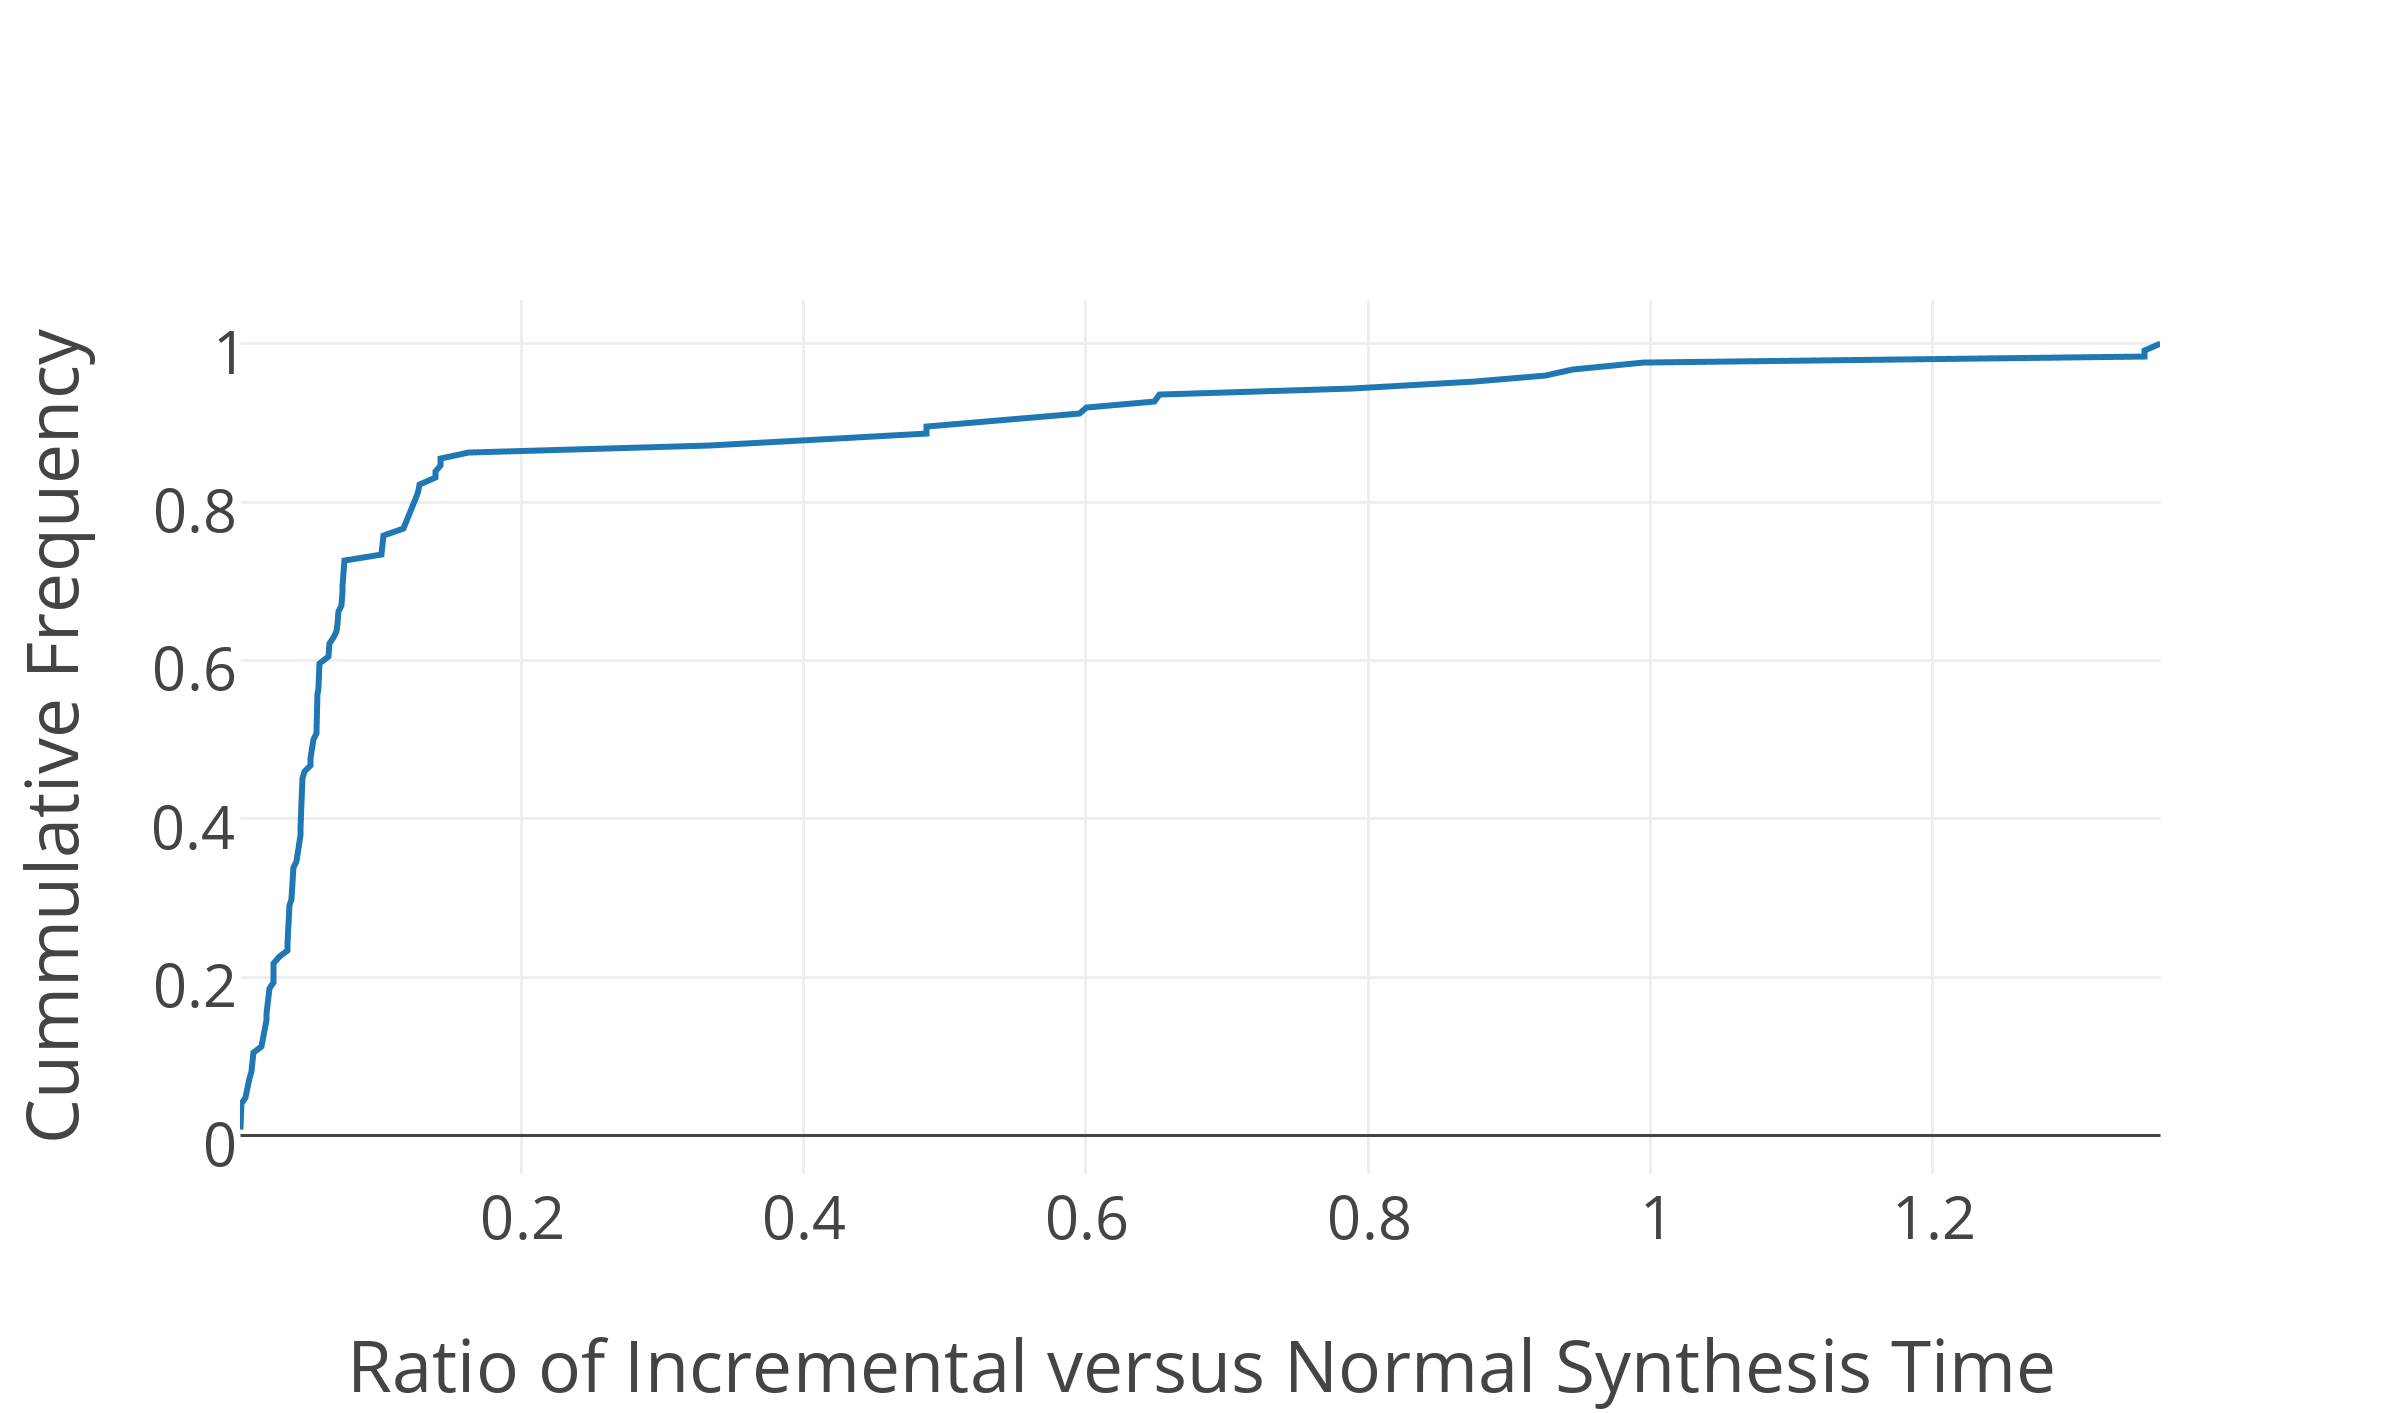
\includegraphics[height=7.5cm]{figures/incremental-cdf.png}
	\caption{Graph used to plot the cummulative frequency for ratio of incremental synthesis/one-shot synthesis.}
	\label{fig:incremental-cdf}
\end{figure*}


%\caption{Synthesis Time for varying number of reachability (with and without tactics) and waypoints policies for a 45 node fat-tree topology}


